\documentclass[12pt]{article}

\usepackage{blindtext} % Package to generate dummy text throughout this template 

\usepackage[utf8]{inputenc}
\usepackage{amsmath, amssymb}
\usepackage{algorithm}
\usepackage{algpseudocode}
\linespread{1.25}
\usepackage[margin = 1in]{geometry}
\usepackage{microtype} % Slightly tweak font spacing for aesthetics
\usepackage[english]{babel} % Language hyphenation and typographical rules
\usepackage{tikz}
\usepackage[hidelinks]{hyperref}
\usepackage{url}
\usepackage{graphicx}
\usepackage{float}
\usepackage{wrapfig}
\usepackage{subcaption}

\setlength{\parindent}{2em}
%\setlength{\parskip}{1.5em}
\graphicspath{ {images/} }

\newcommand{\vect}[1]{\mathbf{#1}}  % vector
\newcommand{\matr}[1]{\mathbf{#1}}  % matrix
\newcommand{\tens}[1]{\mathbf{#1}}  % tensor
\newcommand{\mean}[1]{\overline{#1}}    % mean overline

\begin{document}
    \tableofcontents
    \listoftables
    \listoffigures
    \section{Introduction} \label{sec:Introduction}
    Optimizing predictive models on datasets that are obtained from citizen-science projects can be computationally expensive as these datasets grow in size with time. Consequently, models based on multiple-layered neural networks, Integer Programming and other optimization routines can prove increasingly difficult as the number of parameters increase, despite using the faster Central Processing Units (CPUs) in the market. Incidentally, it becomes difficult for citizen-science projects to scale if the organizers use CPUs to run optimization models. However, Graphical Processing Units (GPUs), which offer multiple cores to parallelize computation, can outperform CPUs in computing such predictive models if these models heavily rely on large-scale matrix multiplications. By using GPUs over CPUs to accelerate computation on a citizen-science project, the model could achieve better optimization in less time, enabling the project to scale.\\
    
    Part of the eBird project, which aims to ``maximize the utility and accessibility of the vast numbers of bird observations made each year by recreational and professional bird watchers'', Avicaching is a incentive-driven game trying to homogenize the spatial distribution of citizens' (agents') observations [cite website]. Since the dataset of agents' observations in eBird is geographically heterogeneous (concentrated in some places like cities and sparse in others), Avicaching homogenizes the observation set by rewarding agents who visit under-sampled locations \cite{Xue2016Avi1}. To accomplish this task of specifying rewards at different locations based on the historical records of observations, Avicaching would learn the change in agents' behavior when a certain sample of rewards were applied to the set of locations, and then distribute a newer set of rewards across the locations based on those learned parameters \cite{Xue2016Avi2}. This requirement naturally translates into a predictive optimization problem, which was implemented using multiple-layered neural networks and linear programming.
    
    \subsection{Identification Problem} \label{sec:Identification Problem}
    As discussed in Section \ref{sec:Introduction}, the model would need to learn parameters that caused the change in agents' behavior when a certain set of rewards was applied to locations in the experiment region. Specifically, given datasets $\vect{y_t}$ and $\vect{x_t}$ of agents' visit densities with and without the rewards $\vect{r_t}$, we want to find weights $\matr{w_1}$ and $\matr{w_2}$ that caused the change from $\vect{x_t}$ to $\vect{y_t}$, factoring in possible influence from environmental factors $\matr{f}$ and distances between locations $\matr{D}$. Although the original model proposed to learn a single set of weights $\matr{w}$ \cite{Xue2016Avi2}, this proposed model considers two sets of weights $\matr{w_1}$ and $\matr{w_2}$ as it may theoretically result into higher accuracy and lower loss. Mathematically, our model can be formulated as:
    \begin{equation} \label{eq:iden_problem}
    \begin{aligned}
    & \underset{\matr{w}}{\text{minimize}}
    & & Z_I(\matr{w_1}, \matr{w_2}) = \sum_{t} (\omega(\vect{y_t} - \matr{P}(\matr{f}, \vect{r_t}; \matr{w_1}, \matr{w_2})\vect{x_t}))^{2}
    \end{aligned}
    \end{equation}
    where $\omega$ is a set of weights at time $t$ capturing penalties relative to the importance of homogenizing at different locations and elements $p_{u, v}$ of $\matr{P}$ are given as:
    \begin{equation} \label{eq:puv_equation}
    p_{u, v} = \frac{\exp(\matr{w_2} \cdot \text{reLU} (\matr{w_1} \cdot [d_{u, v}, \vect{f_{u}}, r_{u}]))}{\sum_{u'} \exp(\matr{w_2} \cdot \text{reLU} (\matr{w_1} \cdot [d_{u', v}, \vect{f_{u'}}, r_{u'}]))} = \frac{\exp(\Gamma_{u, v})}{\sum_{u'}\exp(\Gamma_{u', v})} = \text{softmax}(\Gamma_{u, v})
    \end{equation}
    In the expression for $p_{u,v}$ (Equation \ref{eq:puv_equation}), softmax$(\cdot)$ is the function: softmax$(z_i) = \frac{\exp(z_i)}{\sum_{i}\exp(z_i)}$ and the reLU$(\cdot)$ function is a ``rectified Linear Unit'' defined as: reLU$(z) = \text{max}(0, z)$.
    
    \subsection{Pricing Problem} \label{sec:Pricing Problem}
    After learning the set of weights $\matr{w_1}$ and $\matr{w_2}$ highlighting the change in agents' behavior to collect observations, the Pricing Problem would redistribute rewards to the all locations such that the predicted behavior of agents influenced by the new set of rewards is homogeneous. Thus, given a budget of rewards $\mathcal{R}$, this optimization problem can be expressed as:
    \begin{equation} \label{eq:pricing_problem}
    \begin{aligned}
    & \underset{\vect{r}}{\text{minimize}}
    & & Z_P(\vect{r}) = \frac{1}{n}\lVert \vect{y} - \mean{\vect{y}} \rVert\\
    & \text{subject to}
    & & \vect{y} = \matr{P}(\matr{f}, \vect{r}; \matr{w_1}, \matr{w_2}) \, \vect{x}\\
    &&& \sum_{i} r_i \leq \mathcal{R}\\
    &&& r_i \geq 0
    \end{aligned}
    \end{equation}
    where elements of $\matr{P}$ are defined as in Equation \ref{eq:puv_equation}. 
    
    \subsection{Computation Using GPUs} \label{sec:comp_using_GPUs}
    
    \section{Problem Formulation} \label{sec:Problem Formulation}
    Since NVIDIA General Purpose GPUs enable faster computation on matrices, accelerated through CUDA and cuDNN, both the Identification (Section \ref{sec:Identification Problem}) and the Pricing Problem (Section \ref{sec:Pricing Problem}) were formulated as 3-layered neural networks using the PyTorch library.
    
    \subsection{Design for Identification Problem} \label{sec:Design for Identification Problem}
    To optimize the loss value $Z_I(\matr{w_1}, \matr{w_2})$ (Equation \ref{eq:iden_problem}), the neural network learns the set of weights through multiple iterations of backpropagating the loss using gradient descent. Furthermore, the program would process the dataset before feeding to the network to avoid unnecessary sub-iterations and promote batch operations on matrices. 
    
    \subsubsection{Structure of Input Dataset} \label{sec:Structure of Input Dataset}
    \begin{figure}
        \centering
        \begin{subfigure}{.64\textwidth}
            \centering
            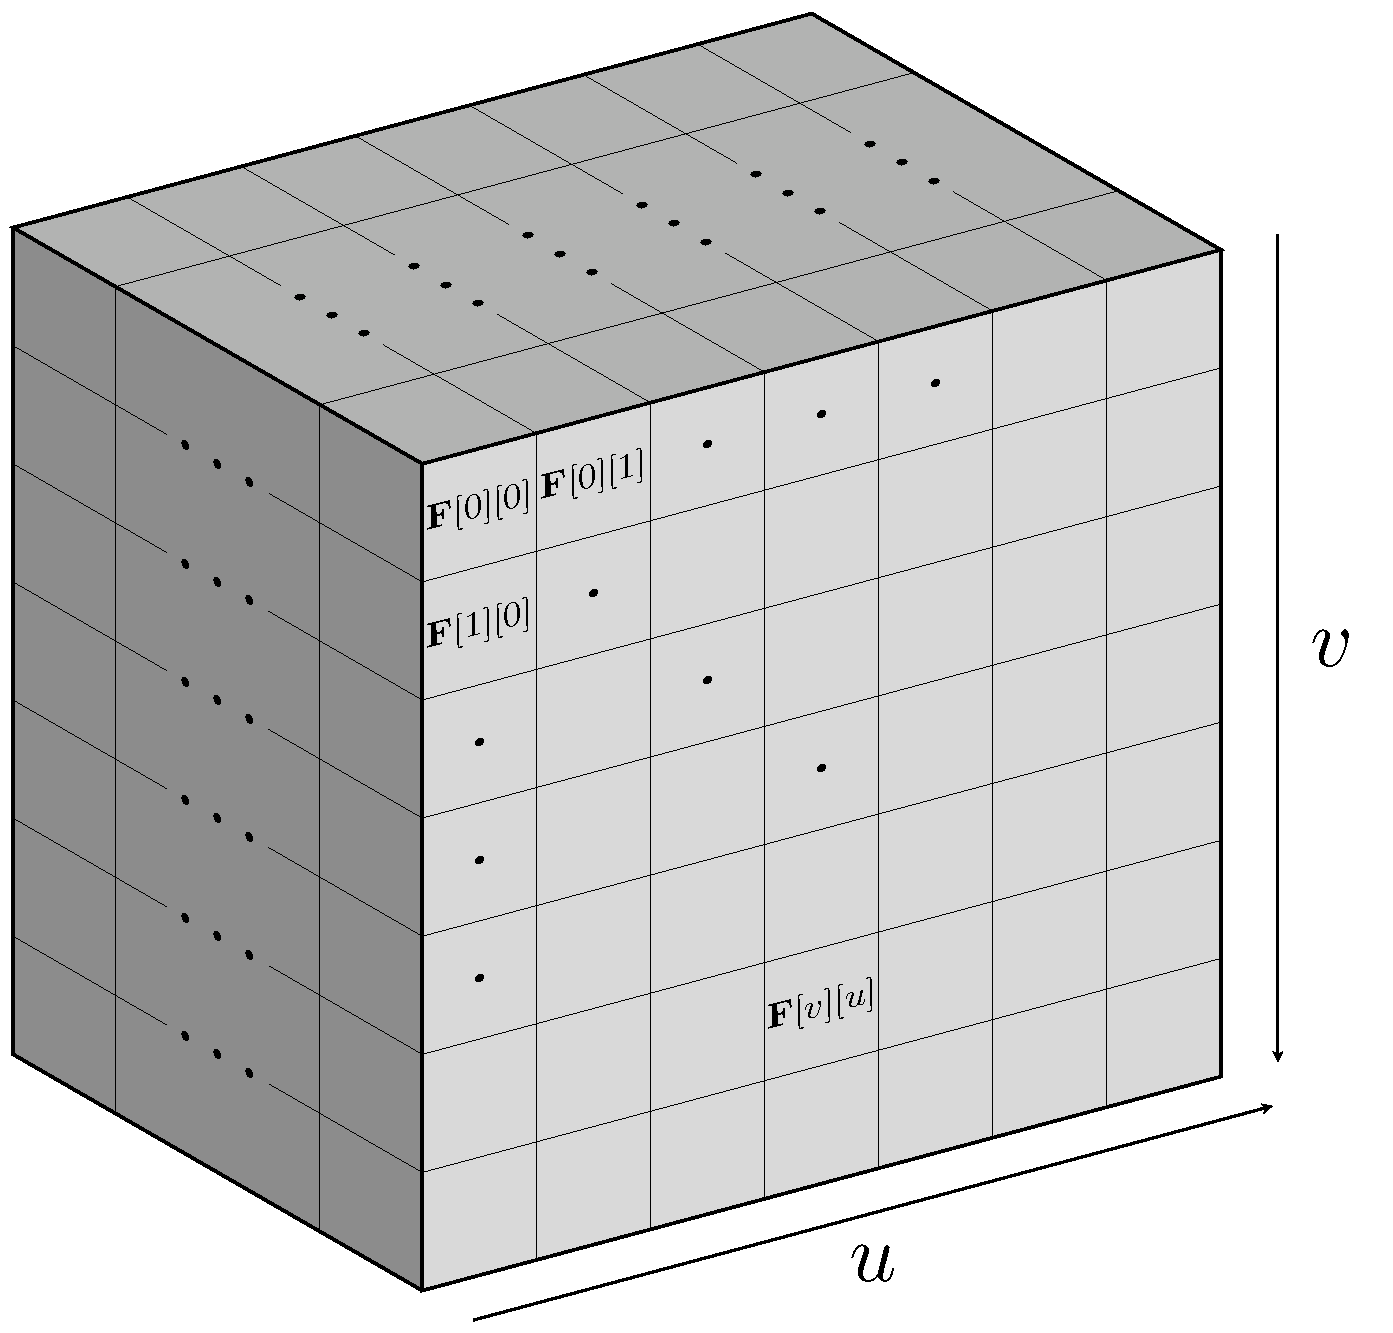
\includegraphics[width=\linewidth]{weights_input_dataset}
            \caption{A Tensor representing the Input Dataset}
            \label{fig:A Tensor representing the complete Input Dataset}
        \end{subfigure}
        \begin{subfigure}{.35\textwidth}
            \centering
            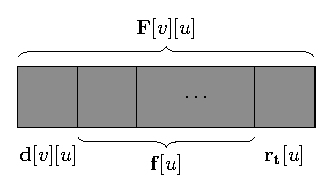
\includegraphics[width=\linewidth]{zoomup_Fuv}
            \caption{Contents of $\vect{F}_{vu}$}
            \label{fig:Zoomed-in contents of Fvu}
        \end{subfigure}
        \caption{Visual representation of the Input Dataset}
        \label{fig:Visual representation of the Input Dataset}
    \end{figure}
    The input dataset comprising of environmental features $\vect{f}$ and given rewards $\vect{r_t}$ must be combined into a tensor (Figure \ref{fig:A Tensor representing the complete Input Dataset}) that can be readily operated on by NVIDIA GPUs. Another advantage of building the dataset as discussed comes with the PyTorch library, which provides convenient handling of tensors residing on CPUs as well as GPUs. Algorithm \ref{alg:Constructing the Input Dataset} describes the steps to construct this dataset.
    \begin{algorithm}
        \caption{Constructing the Input Dataset} \label{alg:Constructing the Input Dataset}
        \begin{algorithmic}[1]
            \State $\matr{d} \gets \Call{Normalize}{\matr{d}}$\Comment{$\matr{d}[u][v]$ is the distance between locations $u$ and $v$}
            \State $\vect{f} \gets \Call{Normalize}{\mathbf{f}, axis = 0}$\Comment{$\mathbf{f}[u]$ is a vector of env. features at location $u$}
            \State $\vect{r_t} \gets \Call{Normalize}{\vect{r_t}, axis = 0}$\Comment{$\vect{r_t}[u]$ is the reward at location $u$}
            \For{$v = 1, 2, \dots J$}
                \For{$u = 1, 2, \dots J$}
                    \State $\tens{F}[v][u] \gets [\matr{d}[v][u], \vect{f}[u], \vect{r_t}[u]]$ \Comment{Looks like Figure \ref{fig:Zoomed-in contents of Fvu}}
                \EndFor
            \EndFor
        \end{algorithmic}
    \end{algorithm}
       
    \subsubsection{Algorithm for Identification Problem} \label{Algorithm for Identification Problem}
    For learning the weights $\matr{w}$ in equation \ref{eq:iden_problem}, a Neural Network was built using the PyTorch library, which minimized the loss function using gradient descent routines. Figure \ref{fig:Neural Network designed for Identification Problem} illustrates the framework of the network used, calculating the vector $\vect{p_v}$. This network was fed in with data from different locations $v$, resulting into the matrix $\matr{P}$, which was then used to calculate the loss.
    \begin{figure}[H]
        \centering
        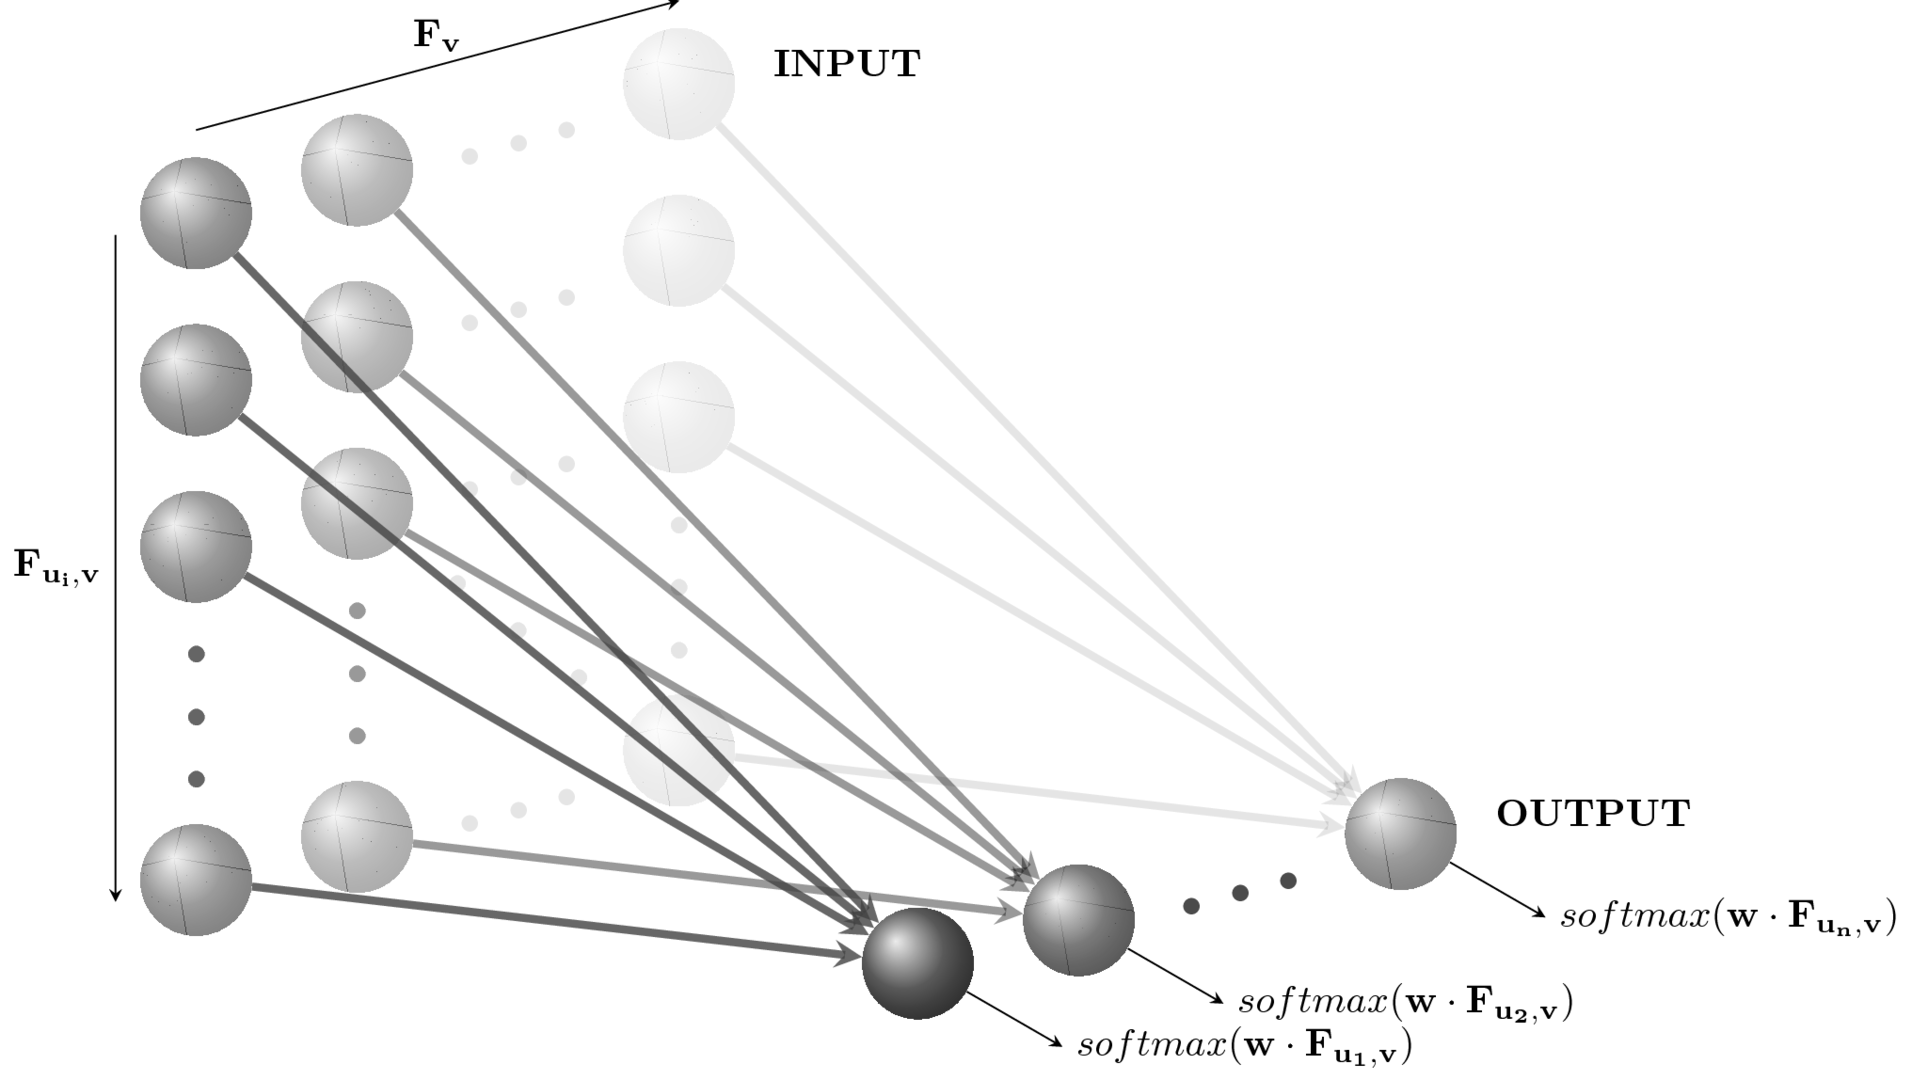
\includegraphics[width=\textwidth]{weights_net}
        \caption{Neural Network designed for Identification Problem}
        \label{fig:Neural Network designed for Identification Problem}
    \end{figure}
    An algorithm for the optimization problem is described in Algorithm \ref{alg:Optimizing for the Identification Problem}.
    \begin{algorithm}
        \caption{Optimizing for the Identification Problem} \label{alg:Optimizing for the Identification Problem}
        \begin{algorithmic}[1]
            \State $a \gets b$
        \end{algorithmic}
    \end{algorithm}
    \section{Experiments}
    
    \section{Results}
    \section{Conclusion}
    
    \blindtext
    \bibliographystyle{ieeetr}
    \bibliography{avicaching}
\end{document}